% THIS TEMPLATE IS A WORK IN PROGRESS
% Adapted from an original template by faculty at Reykjavik University, Iceland

\documentclass{scrartcl}
\usepackage{pdfpages}

% Adapted from an original template by Hlyni Arnórssyni, Reykjavik University, Iceland
%
% ------------------------------ SETTINGS
\usepackage{geometry}

\geometry{
	paper=a4paper, % Paper size
	top=2.5cm, % Top margin
	bottom=2.5cm, % Bottom margin
	left=2.5cm, % Left margin
	right=2.4cm, % Right margin
	headheight=0.75cm, % Header height
	footskip=1.5cm, % Space from the bottom margin to the baseline of the footer
	headsep=0.75cm, % Space from the top margin to the baseline of the header
	%showframe, % Uncomment to show how the type block is set on the page
}

\usepackage{blindtext}
%-------------------------------- Character encoding ----------------------------
\usepackage[T1]{fontenc}
\usepackage[utf8]{inputenc}

%----------------------------- Mathematics packages from AMS ---------------

\usepackage{amsmath, amsfonts, amsthm, amssymb}
\usepackage{braket, nicefrac}

% ----------- International System of Units
\usepackage{siunitx}

%------------------------------ Lists / numbers -------------------------
\usepackage{enumitem, multicol}

%------------------------------- Figure insertions --------------
\usepackage{graphicx, float}  % Use option [H] to force the placement of a figure
\usepackage{keystroke}
\usepackage{pgfplots}\usepgfplotslibrary{units}\pgfplotsset{compat=1.16}

%------------------------------- Line Spacing --------------
\usepackage{setspace}

%------------------------------- Depth of the ToC --------------
\setcounter{tocdepth}{2}

%%%%%%%%%%%%%%%%%%%%%%%%%% Hyperlink References %%%%%%%%%%%%%%%%%%%%%%%%%%%
\usepackage{hyperref}

%--------------------% Storage Path for images %-----------------%
\graphicspath{{graphics/}{Graphics/}{./}}

%%%%%%%%%%%%%%%%%%%%%%%%%% Environments %%%%%%%%%%%%%%%%%%%%%%%%%%%
\renewenvironment{abstract}{
    \begin{center}
    \textbf{Abstract}
    \vspace{0.5cm}
    \par\itshape
    \begin{minipage}{0.8\linewidth}}{\end{minipage}
    \noindent\ignorespaces
    \end{center}
}

\newenvironment{keywords}{
    \begin{center}
    \textbf{Keywords}
    \vspace{0.5cm}
    \par
    \begin{minipage}{0.8\linewidth}}{\end{minipage}
    \noindent\ignorespaces
    \end{center}
}

\newenvironment{preface}{
    \begin{center}
    \textbf{Preface}
    \vspace{0.5cm}
    \par
    \begin{minipage}{0.8\linewidth}}{\end{minipage}
    \noindent\ignorespaces
    \end{center}
}

\newenvironment{acknowledgements}{
    \begin{center}
    \textbf{Acknowledgements}
    \vspace{0.5cm}
    \par
    \begin{minipage}{0.8\linewidth}}{\end{minipage}
    \noindent\ignorespaces
    \end{center}
}
\setlength{\parskip}{1.0\baselineskip} % 

\begin{document}
%Title of the report, name of coworkers and dates (of experiment and of report).
\begin{titlepage}
	\centering
	
\includegraphics[width=0.8\textwidth]{logo.jpg}\par
	\vspace{2cm}
	%%%% COMMENT OUT irrelevant lines among the 3 below
	{\huge\bfseries Title Here\par}  
	\vspace{2cm}
	{\scshape\LARGE By \par}                
	\vspace{1cm}
	{\scshape\LARGE your name here \par}      
	\vspace{0.5cm}
	%{\large \today\par}
	\vspace{1.5cm}
	{\scshape\Large supervised by \par}
	%%%% SUPERVISOR(S)
	\vspace{1cm}
	{\scshape\Large Youmin Xi \\ (Change it here to your supervisor)\par}
	\vspace{3cm}
        %%%% PROJECT TITLE
	{\huge\bfseries Interim Report/Dissertation \par}
	\vfill
	{\scshape\Large YYYY-MM-DD \par}
	\vfill
% Bottom of the page
\end{titlepage}

\newpage
\onehalfspacing

\begin{abstract}

Abstract. Abstract. Abstract. Abstract. Abstract. Abstract. Abstract. Abstract. Abstract. Abstract. Abstract. Abstract. Abstract. Abstract. Abstract. Abstract. Abstract. Abstract. Abstract. Abstract. Abstract. Abstract. Abstract. Abstract. Abstract. Abstract. Abstract. Abstract. Abstract. Abstract. Abstract. Abstract. Abstract. Abstract. Abstract. Abstract. Abstract. Abstract. Abstract. Abstract. Abstract. Abstract. Abstract. Abstract. Abstract. Abstract. Abstract. Abstract. Abstract. Abstract. Abstract. Abstract. Abstract. Abstract. Abstract. Abstract. Abstract. Abstract. Abstract. Abstract. Abstract. Abstract. Abstract. Abstract. Abstract. Abstract. Abstract. Abstract. Abstract. Abstract. Abstract. Abstract. Abstract. Abstract. Abstract. Abstract. Abstract. Abstract. Abstract. Abstract. Abstract. Abstract. Abstract. Abstract. Abstract. Abstract. Abstract. Abstract. Abstract. Abstract. Abstract. 

\end{abstract}
\vspace{1cm}

\begin{keywords}
\centering
 Keywords: \textbf{keywords, keywords, keywords, keywords, keywords, keywords, keywords, keywords, keywords, keywords.}
\end{keywords}

\newpage

%\doublespacing
\tableofcontents
%\singlespacing
\newpage
\onehalfspacing

\section{Introduction}



\newpage

\section{Literature Review}



\subsection{Subsection}

\begin{figure}[H]
	\begin{center}
		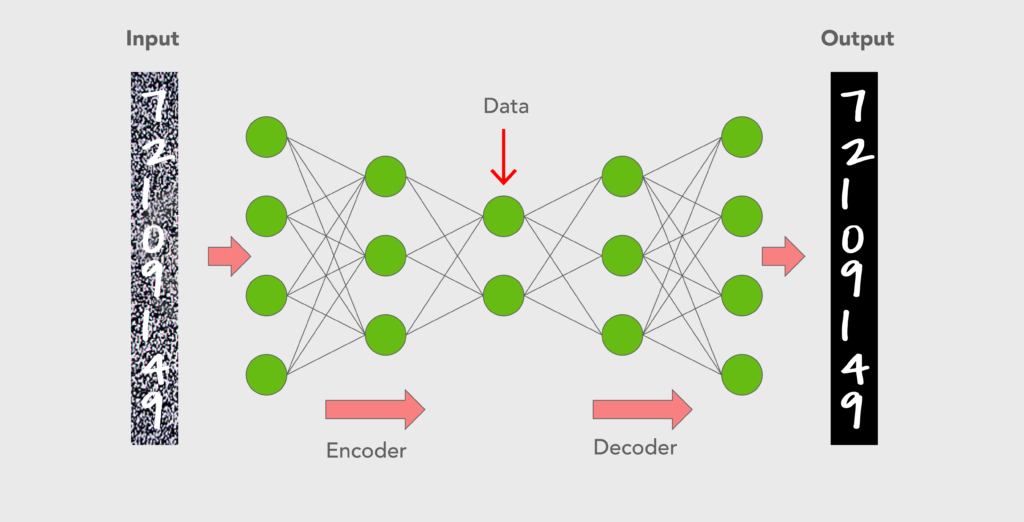
\includegraphics[scale=0.35]{AE.png}
	\end{center}
	\caption{Sample}
	\label{fig:AE}
\end{figure}

The Auto Encoder is a useful tool that can extract high-order data features and work well for nonlinear cases. It also has the ability to compress and denoising data. However, it may not be suitable for handling high-dimensional sparse data, as many hidden units are typically required. This can lead to overfitting, which should be avoided. Its reconstruction error may be too small, making it difficult to learn sparse representation. Since the autoencoder is a non-convex optimization problem, there may be multiple local optima, resulting in the final learned features are not optimized enough. Auto Encoder is sensitive to noise and outliers \cite{cheng2018deep}. The cost function of the Autoencoder is based on reconstruction error, and the model is easy to be disturbed when the input data contains noise or outliers. In addition, the non-convexity and complexity of the model also lead to the need for a large amount of data and original computer training.


\newpage

\section{Problem Statement}


\newpage

\section{Research Methodology}



\neapage

\section{Expected Outcomes and Contributions}


\newpage

\section{Conclusions}



\newpage
\singlespacing
\bibliographystyle{IEEEtran}
\bibliography{references}


%------ To create Appendix with additional stuff -------%

\newpage

\appendix

\section{Appendix  Project Specifications}


%import research proposal here.

% \includepdf[pages={-}]{}


\end{document}
